\documentclass[10pt]{beamer}

% \usepackage{define}
\usepackage{animate}

\usetheme{CCFD}
\usepackage{color}
\definecolor{gray97}{gray}{.90}
\definecolor{gray75}{gray}{.75}
\usepackage{listings}
\lstset{frame=Ltb,
     framerule=0pt,
     aboveskip=0cm,
     framextopmargin=0pt,
     framexbottommargin=0pt,
     framexleftmargin=0cm,
     framesep=0pt,
     rulesep=0pt,
     backgroundcolor=\color{gray97},
     rulesepcolor=\color{black},
     language=C,
           basicstyle=\ttfamily\scriptsize,
           keywordstyle=\color{blue}\ttfamily,
           stringstyle=\color{red}\ttfamily,
           commentstyle=\color{green}\ttfamily,
          breaklines=true,
          }
\lstdefinestyle{consol}
   {basicstyle=\scriptsize\bf\ttfamily,
    backgroundcolor=\color{gray75},
}
\resetcounteronoverlays{lstnumber}

\newcommand{\tabitem}{%
  \usebeamertemplate{itemize item}\hspace*{\labelsep}}

\usepackage{tikz}
\usetikzlibrary{calc,shapes}

\eventtitle{Computer Science I}
\title{Lecture 5 - running in circles}
\date{}

\setbeamertemplate{blocks}[rounded][shadow=true]
\setbeamertemplate{navigation symbols}[]

\begin{document}

\frame{
    \titlepage
}

% \begin{frame}
%   \frametitle{Test is coming}
%   \framesubtitle{28'th November}
%   \begin{itemize}
%     \item Data types
%     \item Functions
%     \item I/O operations
%     \item Branching (if, switch)
%     \item Loops
%   \end{itemize}
% \end{frame}
%
\section{Repeating instructions}

\begin{frame}
  \frametitle{Repeat instructions}
  \begin{columns}
    \begin{column}{0.5\textwidth}
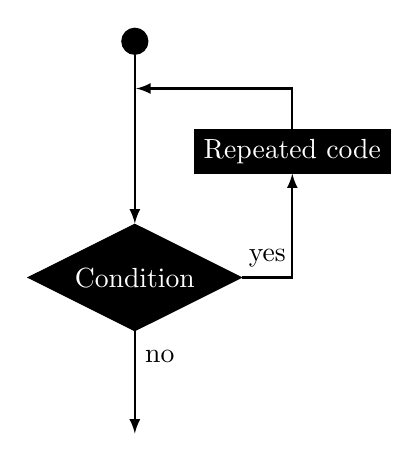
\begin{tikzpicture}[scale=2, node distance = 2cm, auto]
    % Place nodes
    \node [circle, draw, fill=black, minimum size=0.2cm] (A) at (0,0) {};
    \node [inner sep=0pt, outer sep=0pt] (AA) at (0,-0.3) {};
    \node [diamond, draw, fill=black, minimum size=0.2cm, text=white,aspect=2] (B) at (0,-1.5) {Condition};
    \path [draw, -latex, thick] (A) -> (B);
    \node [rectangle, draw, fill=black, minimum size=0.2cm, text=white,aspect=2] (C) at (1,-0.7) {Repeated code};
    \path [draw, -latex, thick] (B) -| node [near start] {yes} (C);
    \path [draw, -latex, thick] (C) |- (AA);
    \node [inner sep=0pt, outer sep=0pt] (BB) at (0,-2.5) {};
    \path [draw, -latex, thick] (B) -> node [near start] {no} (BB);
\end{tikzpicture}
    \end{column}
    \begin{column}{0.5\textwidth}
    \begin{itemize}
      \item Block of code needs to be repeated
      \item Execution is sequential, e.g.: first instruction first, than second ...
      \item Loops allow to execute a statement, or a group of statements a number of times
    \end{itemize}
    \end{column}
  \end{columns}
\end{frame}

\subsection{Bad ideas}

\begin{frame}[fragile]
  \frametitle{Example 1}
  \framesubtitle{Write 100 consecutive numbers ...}

  Bad idea:\\
\begin{lstlisting}
...
printf("%d\n", 0);
printf("%d\n", 1);
printf("%d\n", 2);
...
printf("%d\n", 100);
\end{lstlisting}

\end{frame}

\begin{frame}[fragile]
  \frametitle{GO TO}
  \begin{columns}
    \begin{column}{0.6\textwidth}
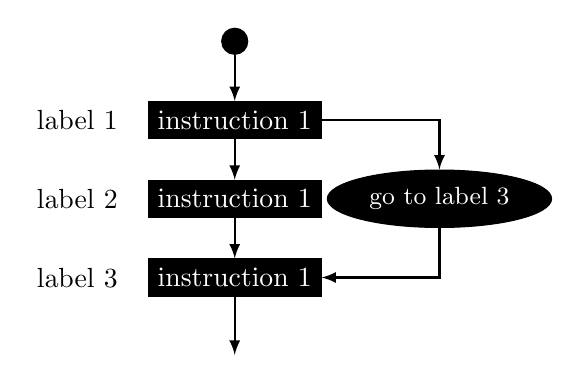
\begin{tikzpicture}[scale=2, node distance = 2cm, auto]
    % Place nodes
    \node [circle, draw, fill=black, minimum size=0.2cm] (A) at (0,0) {};
    \node [inner sep=0pt, outer sep=0pt] (AA) at (0,-0.3) {};
    \node [rectangle, draw, fill=black, minimum size=0.2cm, text=white,aspect=2] (B) at (0,-0.5) {instruction 1};
    \node [] (BB) at (-1,-0.5) {label 1};
    \node [rectangle, draw, fill=black, minimum size=0.2cm, text=white,aspect=2] (C) at (0,-1) {instruction 1};
    \node [] (BB) at (-1,-1) {label 2};
    \node [rectangle, draw, fill=black, minimum size=0.2cm, text=white,aspect=2] (D) at (0,-1.5) {instruction 1};
    \node [] (BB) at (-1,-1.5) {label 3};
    \node [inner sep=0pt, outer sep=0pt] (E) at (0,-2) {};
    \node [ellipse, draw, fill=black, minimum size=0.2cm, text=white,aspect=2] (F) at (1.3,-1) {\small go to label 3 };
    \path[draw, -latex, thick] (A) --(B);
    \path[draw, -latex, thick] (B) --(C);
    \path[draw, -latex, thick] (C) --(D);
    \path[draw, -latex, thick] (D) --(E);
    \path[draw, -latex, thick] (B) -|(F);
    \path[draw, -latex, thick] (F) |-(D);
\end{tikzpicture}
    \end{column}
    \begin{column}{0.5\textwidth}
    \begin{itemize}
      \item Provides a jump to from \textit{goto} to a labeled statment
      \item Although avalible in many languages the use is \textbf{highly discouraged}, and is a mark of poor programming skills
      \item Makes program hard to follow and modify
      \item Any algorithm that uses \textit{goto} can, and should be rewriten to avoid it!
    \end{itemize}
    \end{column}
  \end{columns}
  \begin{center}
    \includegraphics[width=0.7\textwidth, height=0.7\textheight, keepaspectratio]{goto}\\
    {\small XKCD}
  \end{center}

\end{frame}

\begin{frame}[fragile]
  \frametitle{Out first repeated statement}
  \framesubtitle{Better to forget this one!}
  \centering

\begin{lstlisting}
...
int i=0;
start:
printf("%d\n",i);
++i;
if(i<=100) goto start;
...
\end{lstlisting}

\end{frame}

\section{Loops}
\subsection{while}

\begin{frame}[fragile]
  \frametitle{while loop}
  \begin{columns}
    \begin{column}{0.6\textwidth}
\begin{lstlisting}
...
while(condition)
{
  instructions;
}
...
while(condition)
  1 instruction;

\end{lstlisting}
    \end{column}
    \begin{column}{0.5\textwidth}
    \begin{itemize}
      \item Executes as long as condition is \textit{true}
      \item Condition is checked \textbf{befere} execution
      \item ... might not execute at all if condition is \textit{false}!
      \item When finished passes to the line immediately following the loop
    \end{itemize}
    \end{column}
  \end{columns}
\end{frame}

\begin{frame}[fragile]
  \frametitle{while loop}
  \begin{columns}
    \begin{column}{0.6\textwidth}
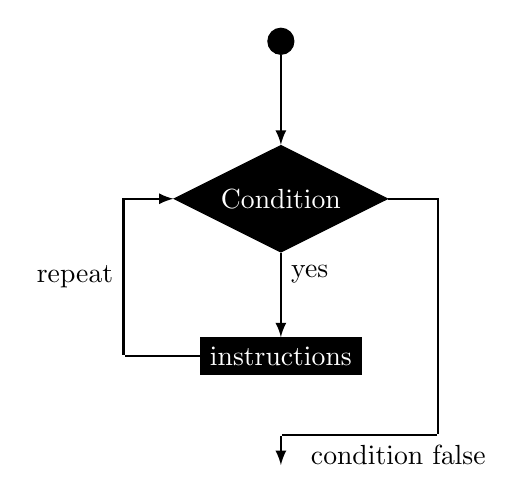
\begin{tikzpicture}[scale=2, node distance = 2cm, auto]
    % Place nodes
    \node [circle, draw, fill=black, minimum size=0.2cm] (A) at (0,0) {};
    \node [diamond, draw, fill=black, minimum size=0.2cm, text=white,aspect=2] (B) at (0,-1) {Condition};
    \node [rectangle, draw, fill=black, minimum size=0.2cm, text=white,aspect=2] (C) at (0,-2) {instructions};
    \node [inner sep=0pt, outer sep=0pt] (CC) at (-1,-2) {};
    \node [inner sep=0pt, outer sep=0pt] (D) at (0,-2.5) {};
    \node [inner sep=0pt, outer sep=0pt] (DD) at (1,-2.5) {};
    \node [inner sep=0pt, outer sep=0pt] (DDD) at (0,-2.7) {};
    \path [draw, -latex, thick] (A) -- (B);
    \path [draw, -latex, thick] (B) -- node [near start] {yes} (C);
    \path [draw, thick] (C) -- (CC);
    \path [draw, -latex, thick] (CC) |- node [near start] {repeat} (B);
    \path [draw, thick] (B) -| (DD);
    \path [draw, thick] (DD) -- node [near start] {condition false} (D);
    \path [draw, -latex, thick] (D) -- (DDD);
\end{tikzpicture}
    \end{column}
    \begin{column}{0.5\textwidth}
    \begin{itemize}
      \item Executes as long as condition is \textit{true}
      \item Condition is checked \textbf{befere} execution
      \item ... might not execute at all if condition is \textit{false}!
      \item When finished passes to the line immediately following the loop
    \end{itemize}
    \end{column}
  \end{columns}
\end{frame}

\subsection{do ... while}

\begin{frame}[fragile]
  \frametitle{do ... while loop}
  \begin{columns}
    \begin{column}{0.6\textwidth}
\begin{lstlisting}
...
do
{
  instructions;
} while(condition)
...
do
  1 instruction;
while(condition)
\end{lstlisting}
    \end{column}
    \begin{column}{0.5\textwidth}
    \begin{itemize}
      \item Executes as long as condition is \textit{true}
      \item Condition is checked \textbf{after} execution
      \item ... executes at leas one time, even if condition is  \textit{false}!
      \item When finished passes to the line immediately following the loop
    \end{itemize}
    \end{column}
  \end{columns}
\end{frame}

\begin{frame}[fragile]
  \frametitle{do ... while loop}
  \begin{columns}
    \begin{column}{0.6\textwidth}
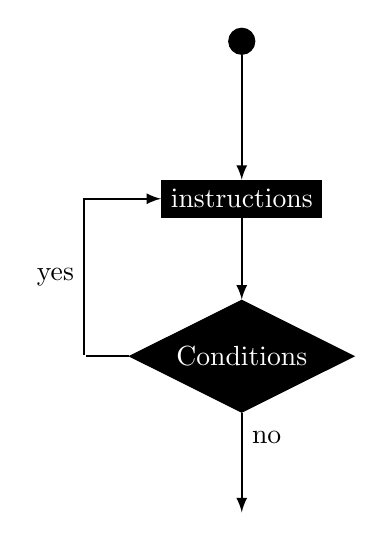
\begin{tikzpicture}[scale=2, node distance = 2cm, auto]
    % Place nodes
    \node [circle, draw, fill=black, minimum size=0.2cm] (A) at (0,0) {};
    \node [rectangle, draw, fill=black, minimum size=0.2cm, text=white,aspect=2] (B) at (0,-1) {instructions};
    \node [diamond, draw, fill=black, minimum size=0.2cm, text=white,aspect=2] (C) at (0,-2) {Conditions};
    \node [inner sep=0pt, outer sep=0pt] (CC) at (-1,-2) {};
    \node [inner sep=0pt, outer sep=0pt] (D) at (0,-3) {};
    \path [draw, -latex, thick] (A) -- (B);
    \path [draw, -latex, thick] (B) -- node [] {} (C);
    \path [draw, thick] (C) -- (CC);
    \path [draw, -latex, thick] (CC) |- node [near start] {yes} (B);
    \path [draw, -latex, thick] (C) -- node [near start] {no} (D);
\end{tikzpicture}
    \end{column}
    \begin{column}{0.5\textwidth}
    \begin{itemize}
      \item Executes as long as condition is \textit{true}
      \item Condition is checked \textbf{after} execution
      \item ... executes at leas one time, even if condition is  \textit{false}!
      \item When finished passes to the line immediately following the loop
    \end{itemize}
    \end{column}
  \end{columns}
\end{frame}

\subsection{for}

\begin{frame}[fragile]
  \frametitle{for}
  \begin{columns}
    \begin{column}{0.6\textwidth}
\begin{lstlisting}
...
for ( init; condition; incr ) {
   instructions
}
...
for ( init; condition; incr )
   instructions
...
for(;;) {} //forever
\end{lstlisting}
    \end{column}
    \begin{column}{0.5\textwidth}
    \begin{itemize}
      \item The \textbf{init} step is executed first, and only once.
      \item ... not requiered as long as ; is in
      \item Condition is checked \textbf{before} execution
      \item ... will not execute if initially condition is  \textit{false}!
      \item \textbf{incr} is performed after the instructions are executed, as a last step,
      \item ... not requiered as long as ; is in
      \item Condition is checked again
      \item ...
    \end{itemize}
    \end{column}
  \end{columns}
\end{frame}

\begin{frame}[fragile]
  \frametitle{for}
  \begin{columns}
    \begin{column}{0.6\textwidth}
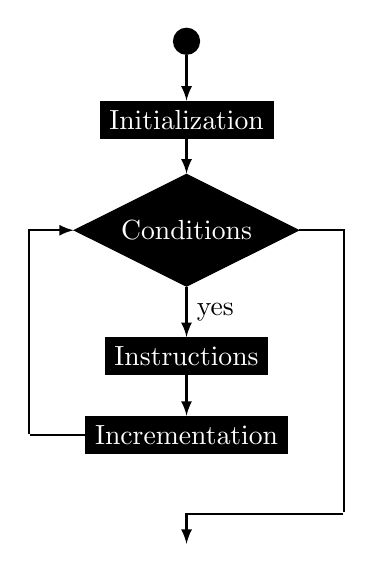
\begin{tikzpicture}[scale=2, node distance = 2cm, auto]
    % Place nodes
    \node [circle, draw, fill=black, minimum size=0.2cm] (A) at (0,0) {};
    \node [rectangle, draw, fill=black, minimum size=0.2cm, text=white,aspect=2] (B) at (0,-0.5) {Initialization};
    \node [diamond, draw, fill=black, minimum size=0.2cm, text=white,aspect=2] (C) at (0,-1.2) {Conditions};
    \node [rectangle, draw, fill=black, minimum size=0.2cm, text=white,aspect=2] (D) at (0,-2) {Instructions};
    \node [rectangle, draw, fill=black, minimum size=0.2cm, text=white,aspect=2] (E) at (0,-2.5) {Incrementation};    
    \node [inner sep=0pt, outer sep=0pt] (CC) at (-1,-2.5) {};
    \node [inner sep=0pt, outer sep=0pt] (DD) at (1,-3) {};
    \node [inner sep=0pt, outer sep=0pt] (DDD) at (0,-3.2) {};
    \path [draw, -latex, thick] (A) -- (B);
    \path [draw, -latex, thick] (B) -- (C);
    \path [draw, -latex, thick] (C) -- node [] {yes} (D);
    \path [draw, -latex, thick] (D) -- (E);
    \path [draw, thick] (E) -- (CC);
    \path [draw, -latex, thick] (CC) |- (C);
    \path [draw, thick] (C) -| (DD);
    \path [draw, -latex, thick] (DD) -| (DDD);
    
\end{tikzpicture}
    \end{column}
    \begin{column}{0.5\textwidth}
    \begin{itemize}
      \item The \textbf{init} step is executed first, and only once.
      \item ... not requiered as long as ; is in
      \item Condition is checked \textbf{before} execution
      \item ... will not execute if initially condition is  \textit{false}!
      \item \textbf{incr} is performed after the instructions are executed, as a last step,
      \item ... not requiered as long as ; is in
      \item Condition is checked again
      \item ...
    \end{itemize}
    \end{column}
  \end{columns}
\end{frame}

\subsection{Nested}

\begin{frame}[fragile]
  \frametitle{Nested loops}
  \framesubtitle{Lopp in a loop in a loop in a ...}
  \begin{columns}
    \begin{column}{0.6\textwidth}
\begin{lstlisting}
...
for ( init; condition; incr ) {
   for ( init; condition; incr ){
    for ( init; condition; incr ){
      instructions
}}}
...
\end{lstlisting}
    \end{column}
    \begin{column}{0.5\textwidth}
    \begin{itemize}
      \item C allows to use loops inside another loops
      \item Can get tricky
    \end{itemize}
    \end{column}
  \end{columns}
\end{frame}

\subsection{Infinite Loop}

\begin{frame}[fragile]
  \frametitle{Infinite Loop}
  \framesubtitle{Loop that runs forever ...}
  \begin{columns}
    \begin{column}{0.6\textwidth}
\begin{lstlisting}
...
for(;;) {} //forever
...
while (true){}
...
\end{lstlisting}
    \end{column}
    \begin{column}{0.5\textwidth}
    \begin{itemize}
      \item The program never ends
    \end{itemize}
    \end{column}
  \end{columns}
\end{frame}

\subsection{Loop Control}

\begin{frame}[fragile]
  \frametitle{break}
  \framesubtitle{Terminates the loop}
  \begin{columns}
    \begin{column}{0.6\textwidth}
\begin{lstlisting}
...
break;
...
\end{lstlisting}
    \end{column}
    \begin{column}{0.5\textwidth}
    \begin{itemize}
      \item The loop is terminated and the code following the loop is executed
    \end{itemize}
    \end{column}
  \end{columns}
\end{frame}

\begin{frame}[fragile]
  \frametitle{continue}
  \framesubtitle{Start the next run immediately}
  \begin{columns}
    \begin{column}{0.6\textwidth}
\begin{lstlisting}
...
continue;
...
\end{lstlisting}
    \end{column}
    \begin{column}{0.5\textwidth}
    \begin{itemize}
      \item The loop execution is stooped, and started from the beginning
    \end{itemize}
    \end{column}
  \end{columns}
\end{frame}

\section{Example with functions}

\begin{frame}[fragile]
  \frametitle{Example with functions}
  \framesubtitle{}
  Write a program, calculating the Fourier expansion of a square wave. Use a function to calculate the values.
    \begin{columns}
    \begin{column}{0.6\textwidth}
  \animategraphics[loop,autoplay,width=\textwidth,poster=first]{3}{something-}{0}{52}
    \end{column}
    \begin{column}{0.5\textwidth}
    \begin{equation}
      f(x)=\frac{4}{\pi} \sum_{n=1}^{\infty}\frac{1}{n}sin(\frac{n\pi x}{L})
    \end{equation}
    \end{column}
  \end{columns}

  
\end{frame}
\end{document}
